\subsection{Design Language}
This section will use the physical design process, in which the prototypes and the conceptual model are combined, to produce the design language for the program. The physical design process is concerned with defining the look and feel of the program. The process also defines the allocation of functions and the knowledge between a user and a device. The product, which is the design language, is a standardization of the interaction with the program and the physical style of the program e.g. buttons, shapes, colours. This means that the design language is a guide line during the development phase but that the actual program can differentiate itself from the design language.

\subsubsection{Program Screens and Functionality} \label{ScreensandFunctionality}
The domains were identified in \cref{ScenarioCorpus} and they are as follows: planning, shopping, recipes, inventory and general. In \nameref{Sketches} the domains were used to structure the screens in the program. In the \nameref{ConsMod} the domains were used as main elements. Because of the structural contribution that the domains give they will be used as a basis for the actual screens of the program. The following text will describe each screen of the program by the funcionalities of the particular screen.

\paragraph{Planning}
By first looking at the \nameref{ConsMod} we see that there are some functional requirements stated for the Meal Planner. The requirements are listed below.

\begin{itemize}
\item Recipes planned for a dynamic number of people.
\item Varied meals.
\item Change meal Plans on the fly.
\end{itemize}  

By also looking at the \nameref{Sketches} and more specifically in \cref{MealScheduleSketches} we can add to the list of requirements. The additions are listed below.

\begin{itemize}
	\item A weekly overview of planned meals.
		\begin{itemize}
			\item With information  for each meal e.g. name of the recipe, date and number of ingredients the user has.
		\end{itemize}
	\item A view of a specific day and the planned recipes.
		\begin{itemize}
			\item Display the current selected day the user is viewing.
			\item A way to add a meal to the day.
			\item A way to edit already scheduled meals.
		\end{itemize}  
\end{itemize} 

\paragraph{Shopping}
By also looking at the \nameref{ConsMod} for this screen we can identify different functional requirements. The requirements are listed below.

\begin{itemize}
	\item Dynamic number of days to shop for.
	\item Shared list.
	\item Automatically add bought items to inventory.
	\item Meal plan changes effects the shopping list.
\end{itemize} 

By also looking at the \nameref{Sketches} and more specifically in \cref{ShoppingListSketches} we can add to the list of requirements. The additions are listed below.

\begin{itemize}
	\item An overview of all ingredients on the shopping list.
		\begin{itemize}
			\item Displaying each ingredients name and quantity.
		\end{itemize}		 
	\item A search function to find and add specific ingredients.
	\item A function to buy or add ingredients to the inventory.	
\end{itemize}

\paragraph{Recipes}
The \nameref{ConsMod} also states different functional requirements for this screen. The requirements are listed below.

\begin{itemize}
	\item Ingredients.
		\begin{itemize}
			\item Displaying name and quantity of the ingredients.
		\end{itemize}
	\item Preparation
		\begin{itemize}
			\item An explanation of cooking steps for the specific recipe.
		\end{itemize}
	\item Diets
\end{itemize} 

The list can be expanded with the functional requirement from \nameref{Sketches}, specific in \cref{RecipesSketches}

\begin{itemize}
	\item A search function.
	\item A list of recipes with little but relevant information.
		\begin{itemize}
			\item Information could be a picture of the recipe, recipe name, ingredients of the recipe and the number of ingredients the user has.
		\end{itemize}
	\item A categorization function
	\item A view of a specific recipe.
		\begin{itemize}
			\item Information such as preparation guide, ingredients and a picture.
			\item A function add the recipe to the meal schedule.
		\end{itemize}
\end{itemize}

\paragraph{Inventory}
The \nameref{ConsMod} States different functionalities requirements for the inventory screen. These requirements are listed below.

\begin{itemize}
	\item A function to manually add ingredients.
	\item Automatic adding of bought shopping list ingredients.
\end{itemize}

The additions to the functional requirements from \nameref{Sketches} and more \cref{RecipesSketches} are listed below.

\begin{itemize}
	\item A search function to find and add specific ingredients.
	\item A function to remove ingredients.
	\item A list of ingredients with little but relevant information.
		\begin{itemize}
			\item Information such as Ingredient name, purchase date and quantity.
		\end{itemize}
	\item A function or view that easily groups ingredients of the same name but has different quantities and/ or purchase dates.
\end{itemize}  

\paragraph{General}   
The \nameref{ConsMod} does not include this domain and the design requirements will therefore be identified from the \nameref{Sketches}. The design requirements are listed below.

\begin{itemize}
	\item An overview of all the different setting categories.
		\begin{itemize}
			\item Categories such as Stock, allergies, preferences and more.
		\end{itemize}
	\item A function to expand and display specific categories and the information for that category.
\end{itemize} 
 
\subsubsection{Program Navigation}
The main method of the navigation in the program is done via the bottom navigation bar shown on \cref{NavigationBarSketch}. This bar can be used from all the screens of the program and directs the user to one of the five main screens written above in \textit{Program Screens and Functionality}. If the user navigates away from one of the main screens, e.g. when viewing a list of recipes the user could press a recipe and view that specific recipe, the top of the screen will give a back functionality. 

\subsubsection{Design Principles}
This section will discuss different design subjects that are used as general principles in the design language for the program. These general principles are made to give the programs design coherence and by doing so increase the usability. 

The navigation in the program is mainly done via the bottom navigation bar. Consistently displaying and using this as the main way of navigation gives the program better usability. If the user is confused as to where he is in the program he can always use the bottom navigation bar to find his way to a screen that is familiar. Another consistency that the programs navigation has is the use of the top navigation bar. When the user is on any screen that is not one of the main screens the top bar will be used as a backwards navigation. The consistency of using both the bottom and top for navigation functions gives an easy of use and better usability.

The program will be designed as a mobile application. It is therefore important that this is considered when defining more general principles for the program. These additional principles are listed and briefly described below.

\begin{itemize}
	\item General
		\begin{itemize}
			\item Try to avoid to much redundant information on the screen
			\item Avoid to many click function and mouseover functions.
		\end{itemize}
	\item Text
		\begin{itemize}
			\item The text has to be readable. That means using logical typography e.g. giving it the right size relative to the screen and an easy to read font.	
			\item the use of font and text size has to be consistent.
		\end{itemize}
	\item Buttons
		\begin{itemize}
			\item The shape and color theme has to be consistent on buttons.
			\item The size of the buttons has to be larger enough for a person to click with a finger.
			\item Avoid to much text on the buttons. A good idea is to use icons.
			\item Avoid using buttons when it is not necessary e.g. When editing an ingredient the program should update automatically.
		\end{itemize}
\end{itemize}    

\paragraph{Colour Choice}

In order to make to program more appealing, colours are used in the design. It is important that the colours give the right statement, and that they seem attractive to the user.

The colour that was discussed first, using Paletton, was a red colour. This was supposed to be the colour of headlines and such in the program. The reason for discussing red is that red indicates appetite and food\cite{color_psychology}. Red was not chosen though, as it is too strong of a colour, and this might put the user off as it can also indicate danger or alerts.

Since red was not the optimal choice of colour, orange was considered for its similarity to red. Orange has the same quality of red to encourage appetite for the user. Furthermore is orange also a cheerful colour, and it was found to be very appealing, lastly it may be used in the program without standing out too much, or give the user wrong impressions.

\begin{figure}[H]
	\centering
    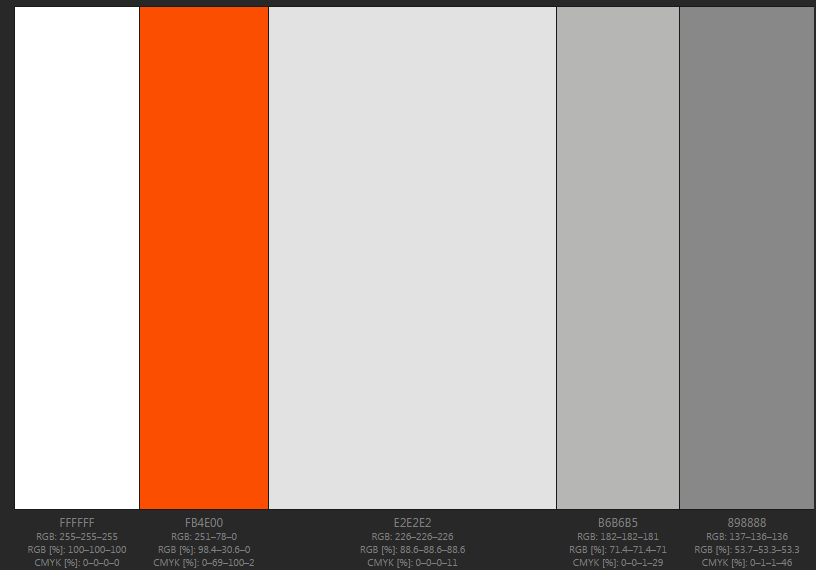
\includegraphics[width=0.9\textwidth]{Grafik/FoodPlanner/ChosenColours}
	\caption{The chosen colours for the software}
	\label{ChosenColours}
\end{figure}
\fxnote{cut some of the top of this fig. + maybe put numbers 1 to 5 on the colours, and refer to these, and not only the hashcode}
The shade of orange and a range of gray colours were chosen, and can be seen in \cref{ChosenColours}.

The colour \#898888 is used for the borders of the program. If something is parted, or a button needs a border, this colour is used. The reason for choosing this colour is that it is much darker than the other colours and gives a clear indication of an ending item.

The colour \#FB4E00 is the orange colour as can be seen in \cref{ChosenColours}. This colour is the one used for the headline text, as is the main colour of the program, since it is the only colour that can't be characterized as a neutral colour. It is only used for the headline text, as it would be difficult for the user to read the text if it was all orange.

The colour \#E2E2E2 is used for the background of the software. This is a very light colour, and it is easy to read black text on it, furthermore does the orange headlines stand more sharp, which makes them easier to see. Therefore this colour was chosen for the background. The white colour \#FFFFFF was also considered, but it was too light, and might irritate the user, lastly it did not go as well with the borders as \#E2E2E2.

